\documentclass{beamer}
% \usepackage[utf8]{inputenc}
\usepackage{amsmath}
\usepackage{amssymb}
\usepackage{amsfonts}
\usepackage{bbm}
\usepackage{tikz}
\usetikzlibrary{positioning}
\usepackage{subcaption}
\captionsetup{compatibility=false}

% \usepackage[pdftex]{graphicx}
\graphicspath{{images/}}

\tikzset{set/.style={draw,circle,inner sep=0pt,align=center}}

\usepackage{appendixnumberbeamer}

\usetheme[sectionpage=progressbar,subsectionpage=progressbar,numbering=fraction,
          progressbar=foot]{metropolis}

\title{Optimization: Stochastic Gradient Descent}
\subtitle{Convolutional Neural Networks for Visual Recognition\\
\url{http://cs231n.github.io/}}

\usepackage{datetime}
\newdate{seminardate}{07}{07}{2017}

\date{\displaydate{seminardate}}
\author{%
  Simon Bihel, \url{simon.bihel@ens-rennes.fr} \\
}
\institute{%
  COINSE Lab, KAIST% \\
  % University of Rennes I \\
  % École Normale Supérieure de Rennes
}

\begin{document}

\maketitle

\begin{frame}{Table of contents}
  \setbeamertemplate{section in toc}[sections numbered]
  \tableofcontents[hideallsubsections]
\end{frame}


\section{Introduction}
\begin{frame}
  \frametitle{Last week with Jinhan}
  A \textbf{score function} mapping the raw image pixels to class scores, e.g.
  \[f(x_i, W) =  W x_i\]
  With $W$ being a set of parameters.

  A \textbf{loss function} measuring the quality (how the scores agree with training data) of a set of parameters, e.g. SVM
  \[L = \frac{1}{N} \sum_i \sum_{j\neq y_i} \left[ \max(0, f(x_i; W)_j - f(x_i; W)_{y_i} + 1) \right] + \alpha R(W)\]

  We want to minimize the loss function by tweaking $W$.
\end{frame}

\begin{frame}
  \frametitle{Visualizing the loss function}
  Difficult to visualize due to high-dimensional spaces. Gain some intuition by choosing a random $W$ and moving in a random direction ($L(W + a W_1)$) \visible<2->{or 2 directions ($L(W + a W_1 + b W_2)$).}
  \begin{figure}
    \begin{subfigure}{.33\textwidth}
      \centering
      \visible<1->{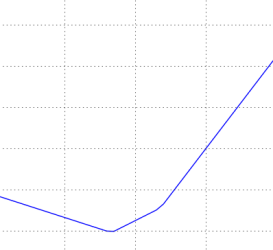
\includegraphics[width=.95\textwidth]{svm1d}}
      \visible<1->{\center{1 dim, 1 example}}
    \end{subfigure}%
    \begin{subfigure}{.33\textwidth}
      \centering
      \visible<2->{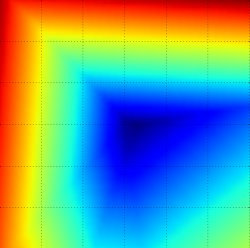
\includegraphics[width=.95\textwidth]{svm_one}}
      \visible<2->{\center{2 dim, 1 example}}
    \end{subfigure}%
    \begin{subfigure}{.33\textwidth}
      \centering
      \visible<3->{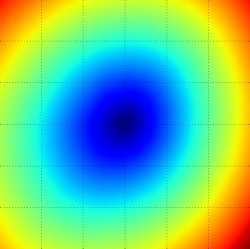
\includegraphics[width=.95\textwidth]{svm_all}}
      \visible<3->{\center{2 dim, 100 examples}}
    \end{subfigure}%
  \end{figure}
\end{frame}

\begin{frame}
  \frametitle{Piecewise-linear structure of the loss function}
  For a single example we have
  \[L_i = \sum_{j\neq y_i} \left[ \max(0, w_j^Tx_i - w_{y_i}^Tx_i + 1) \right]\]
  \begin{center}
    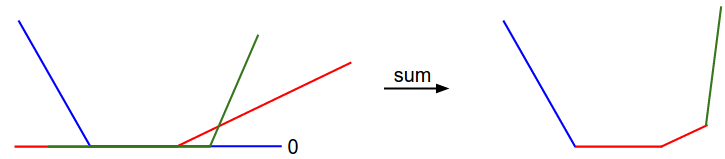
\includegraphics[width=0.8\textwidth]{svmbowl}
  \end{center}
  \vfill{}
  In our examples the loss function is convex but it is not in practice with neural networks, thus we need more general minimization techniques.
\end{frame}


\section{Optimization}
\begin{frame}
  \frametitle{Strategy \#1: Random Search}
  Obviously not the most accurate method on its own. But it is a good starting point to iteratively refine it.
\end{frame}

\begin{frame}
  \frametitle{Strategy \#2: Random Local Search}
  Start from a random $W$ and add a random perturbation $W + \delta W$ and perform an update if the loss is lower.

  Still wasteful and computationally expensive.
\end{frame}

\begin{frame}
  \frametitle{Strategy \#3: Following the gradient}
  No need to randomly search for a good direction: we can compute the \textit{best} direction with the steepest descend. This direction is called the \textbf{gradient} of the loss function

  The gradient is just a vector of slopes (i.e.\ \textbf{derivatives})

  For a 1-D function it is:
  \[\frac{df(x)}{dx} = \lim_{h\ \to 0} \frac{f(x + h) - f(x)}{h}\]
  For vectors it is simply the vector of derivatives for each dimension (called \textbf{partial derivatives})
\end{frame}


\section{Computing the gradient}
\begin{frame}
  \frametitle{Numerically with finite differences}
  Slow, approximate but easy way.

  For each dimension, make a small change and compute the partial derivative along that dimension.

  Choosing the step size (aka \textit{learning rate}) is one of the most important hyperparameter in training a NN. Large changes can miss minimums but are faster.
\end{frame}

\begin{frame}
  \frametitle{Analytically with calculus}
  Derive a direct formula for the gradient. No approximations and very fast to compute but error-prone in the implementation.

  Lets use the example of the SVM loss function for a single datapoint:
  \[L_i = \sum_{j\neq y_i} \left[ \max(0, w_j^Tx_i - w_{y_i}^Tx_i + \Delta) \right]\]

  \[\nabla_{w_{y_i}} L_i = - \left( \sum_{j\neq y_i} \mathbbm{1}(w_j^Tx_i - w_{y_i}^Tx_i + \Delta > 0) \right) x_i\]

   You can check the correctness by comparing with the numerical gradient (\textbf{gradient check}).
\end{frame}

\begin{frame}
  \frametitle{Gradient descent}
  It is the procedure of repeatedly evaluating the gradient and then performing a parameter update. This is the core of all NN libraries.

  For large training data, a common approach is to compute the gradient over \textbf{batches} of data. This works well because training data are correlated.

  \textbf{Stochastic Gradient Descent (SGD)} is the process of computing the gradient multiple times for only one example.
\end{frame}


% \section*{Conclusion}
% \begin{frame}
%   \frametitle{Summary}
%   \begin{center}
%     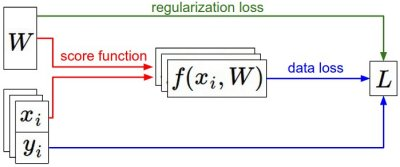
\includegraphics[width=0.9\textwidth]{dataflow}
%   \end{center}
% \end{frame}

\end{document}
